
   %%%%%%%%%%%%%%%%%%%%%%%
 %%%  NOAH'S SUPER COOL  %%%
%%%%      ACADEMIC       %%%%
 %%%   LATEX TEMPLATE    %%%
   %%%%%%%%%%%%%%%%%%%%%%%

\documentclass[12pt]{article}
\usepackage[letterpaper]{geometry}
\geometry{top=1in, bottom=1in, left=1in, right=1in}
\usepackage{fontspec}
\usepackage{tgtermes}
\usepackage{hanging}
\usepackage{hyperref}
\setmainfont[
 ItalicFont={texgyretermes-italic.otf},
 BoldFont={texgyretermes-bold.otf},
 ]{texgyretermes-regular.otf}
\usepackage{setspace}
\doublespacing
\usepackage{graphicx}
\graphicspath{ {./} }

\begin{document}

\setlength{\parindent}{0in}
SPA 4 - Part A \\ Noah Dinan \\ CSC 2210 - Bhattacharya \\ \today \\
\textbf{repository:} \url{https://github.com/shinysocks/csc2210/tree/main/morsecoder}

\vspace{0.2in}

\pagenumbering{arabic} % resume page numbering

morsecoder is a prototype for a game project to "gamify" decoding morse code from user input.

The core game engine being used to handle keyboard events, visuals, and timing is raylib.

The MorseTree class stores each morsecode sequence within a binary tree path.

\begin{center}
    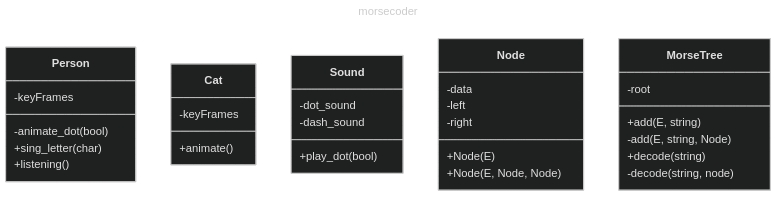
\includegraphics[scale=0.6]{o-1.png}
\end{center}

\begin{center}
    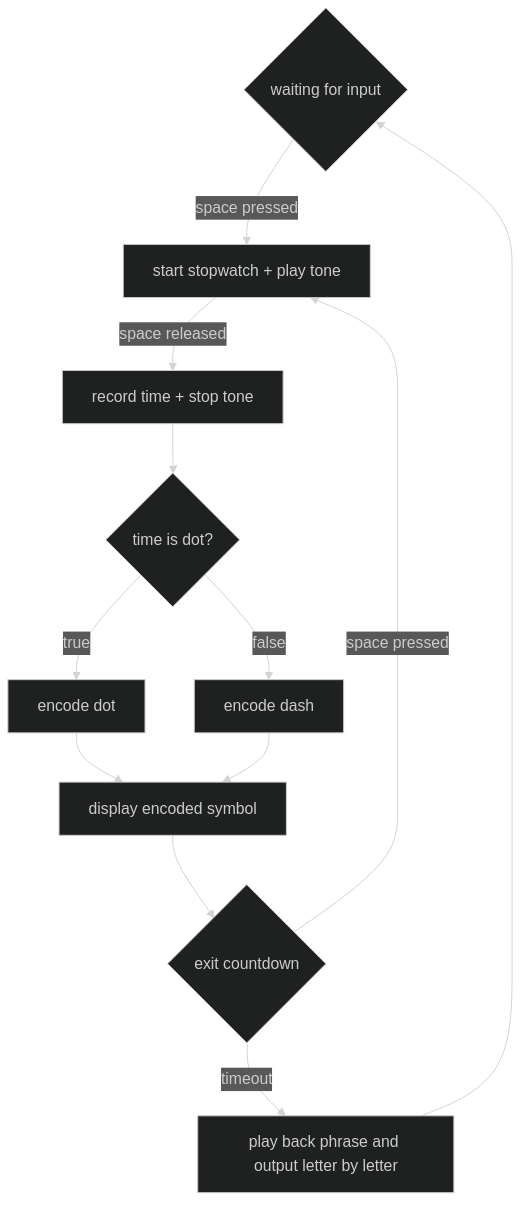
\includegraphics[scale=0.5]{o-2.png}
\end{center}

\end{document}
